\subsection{Sensitivity Test}
Based on the analysis above, we modify the Multi-groups Logistic Model.
\begin{equation}
  \begin{cases}
    \frac{1}{N_x(t)}\frac{dN_x(t)}{dt} = r_x(t)(1-\frac{N_x(t)}{{{N'}_x}_{max}} - RGB_x\frac{N_y(t)}{{{N'}_y}_{max}}) \\ \\
    \frac{1}{N_y(t)}\frac{dN_y(t)}{dt} = r_y(t)(1-\frac{N_y(t)}{{{N'}_y}_{max}} - RGB_y\frac{N_x(t)}{{{N'}_x}_{max}})
  \end{cases}
\end{equation}
\par
We take $F_A$ and $F_B$ as examples to analyze the sensitivity of our model when environment fluctuates rapidly. Because they are all drought-tolerant fungi, when rapid fluctuations in the environment have an adverse effect, they will appear as heavy precipitation in a short period of time. We artificially set rapid fluctuations in the environment on the fifth day and draw curve figure of $N_A'(t)$ and $N_B'(t)$ as follows.
\begin{figure}[H]
  \centering
  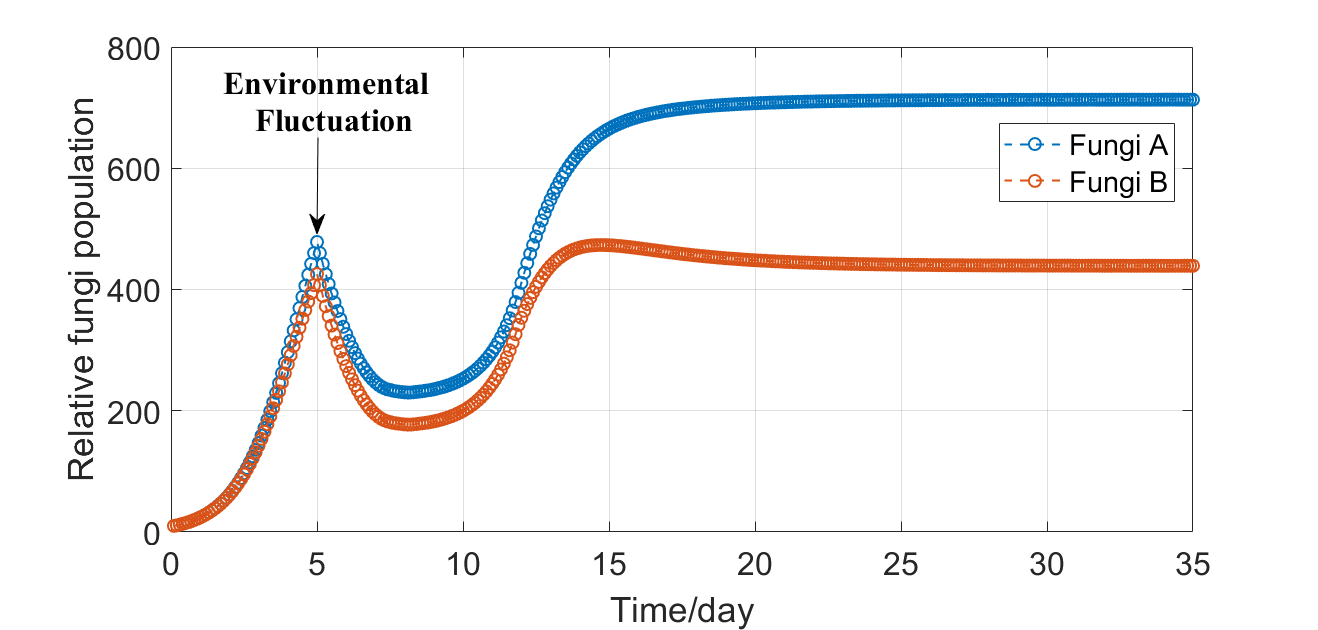
\includegraphics[width=\textwidth]{figures/A&B_sen.png}
  \caption{Curves of $N_A'(t)$ and $N_B'(t)$.}
\end{figure}
\par
From the above figure, it is found that the fungal population maintained an exponential growth in the first $5$ days. After rapid environmental fluctuations occurred on the $5th$ day, the populations of $F_A$ and $F_B$ both declined significantly. Around the $11th$ day, the population began to increase. After $20$ days, the populations of $F_A$ and $F_B$ both stabilized, at $713$ and $439$, respectively. Compared with the stable fungal population of $F_A$ and $F_B$ without the influence of rapid environmental fluctuations, the values have dropped by $10.4\%$ and $15.9\%$, respectively.
\par
Therefore, when rapid environmental fluctuations occur, the \textbf{advanced Multi-groups Logistic Model} could well reflect the influence of harsh environments on the growth and reproduction of fungi, which shows that the model has \textbf{good sensitivity}.